%%%%             %%%%
%%%% ADICIONAL 1 %%%%
%%%%             %%%%

\chapter{Imágenes y código adicional}
\label{chap:adicional-1}

\lettrine{E}{n} este apéndice se presentan imágenes y código adicionales que por su tamaño no se incluyen en el cuerpo de la memoria.

% TODO añadir imágenes de los documentos tratados

\begin{figure}[hp!]
    \centering
    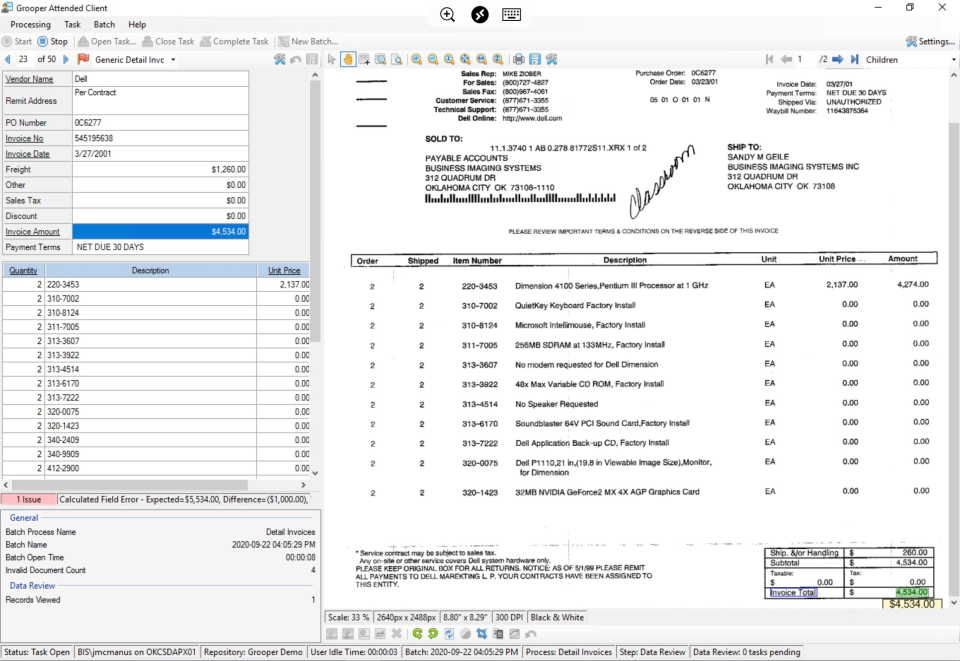
\includegraphics[width=0.9\textwidth]{imaxes/b-estado-arte/bisok-grooper}
    \caption{Grooper, la solución de Bisok}
    \label{fig:grooper-bisok}
\end{figure}

\begin{figure}[hp!]
    \centering
    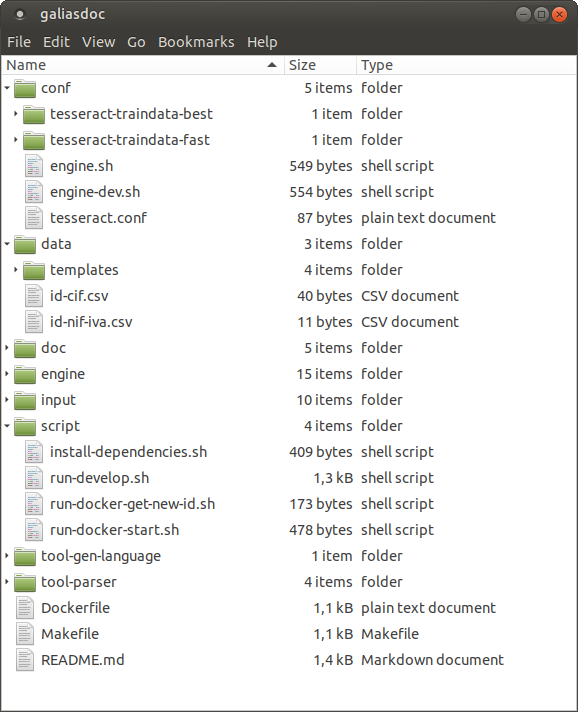
\includegraphics[width=0.8\textwidth]{imaxes/z-adicional/estructura-general.png}
    \caption{Vista general de los directorios del proyecto}
    \label{fig:directorios-proyecto}
\end{figure}

\begin{figure}[hp!]
    \centering
    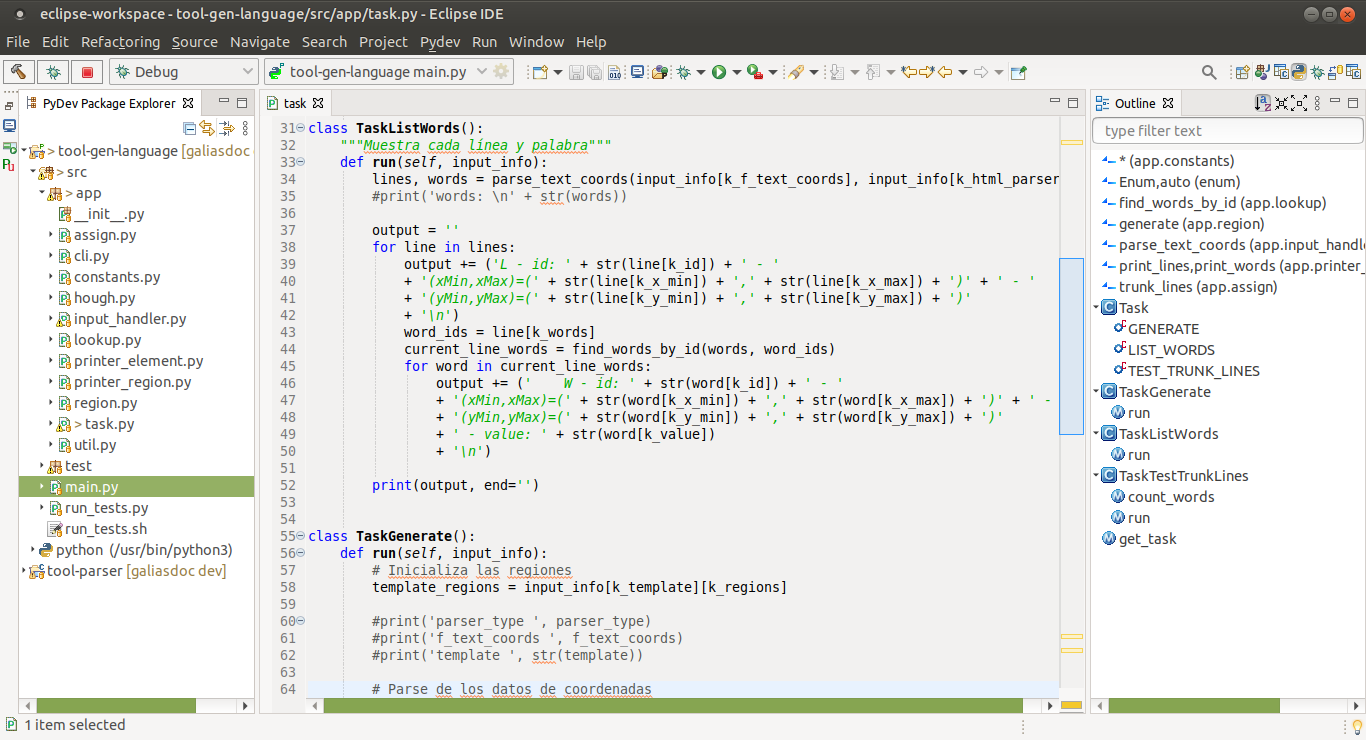
\includegraphics[angle=90,height=1.6\textwidth]{imaxes/z-adicional/tool-gen-language-pydev.png}
    \caption{Eclipse Pydev con el generador de código intermedio}
    \label{fig:tool-gen-language-pydev}
\end{figure}

\noindent\begin{minipage}{.45\textwidth}
\begin{lstlisting}[caption=Scripts del \emph{engine}]{ScriptsEngine}
engine/
    extract-images.sh
    extract-text-coords.sh
    extract-text.sh
    fix-page-numbers.sh
    generate-images-for-text-based.sh
    generate-json.sh
    get-job-id.sh
    identify-grep.sh
    image-apply-blur.sh
    image-apply-ocr.sh
    image-apply-unskew.sh
    populate-result.sh
    run.sh
    split-text-from-image.sh
    unpack.sh
\end{lstlisting}
\end{minipage}\hfill
\begin{minipage}{.45\textwidth}
\begin{lstlisting}[caption=Fuentes del procesador de lenguaje intermedio,label=lst:fuentes-del-procesador-de-lenguajes]{ProcesadorLenguajes}
tool-parser/
    Makefile
    lib/
        cJSON.c
        cJSON.h
        lista.c
        lista.h
        reg-exp.c
        reg-exp.h
        strbuf.c
        strbuf.h
        util.c
        util.h
    main/
        app-conf.h
        bison-epilogue.c
        bison-epilogue.h
        bison-prologue.c
        bison-prologue.h
        flex-prologue.c
        flex-prologue.h
        gen-amount.c
        gen-amount.h
        gen.c
        gen.h
        global-vars.h
        main.c
        main.h
        types.h
    plugin/
        A48941488.l
        A48941488.y
        B15035801.l
        B15035801.y
        B83834747.l
        B83834747.y
        IE6364992H.l
        IE6364992H.y
\end{lstlisting}
\end{minipage}

\begin{figure}[hp!]
    \centering
    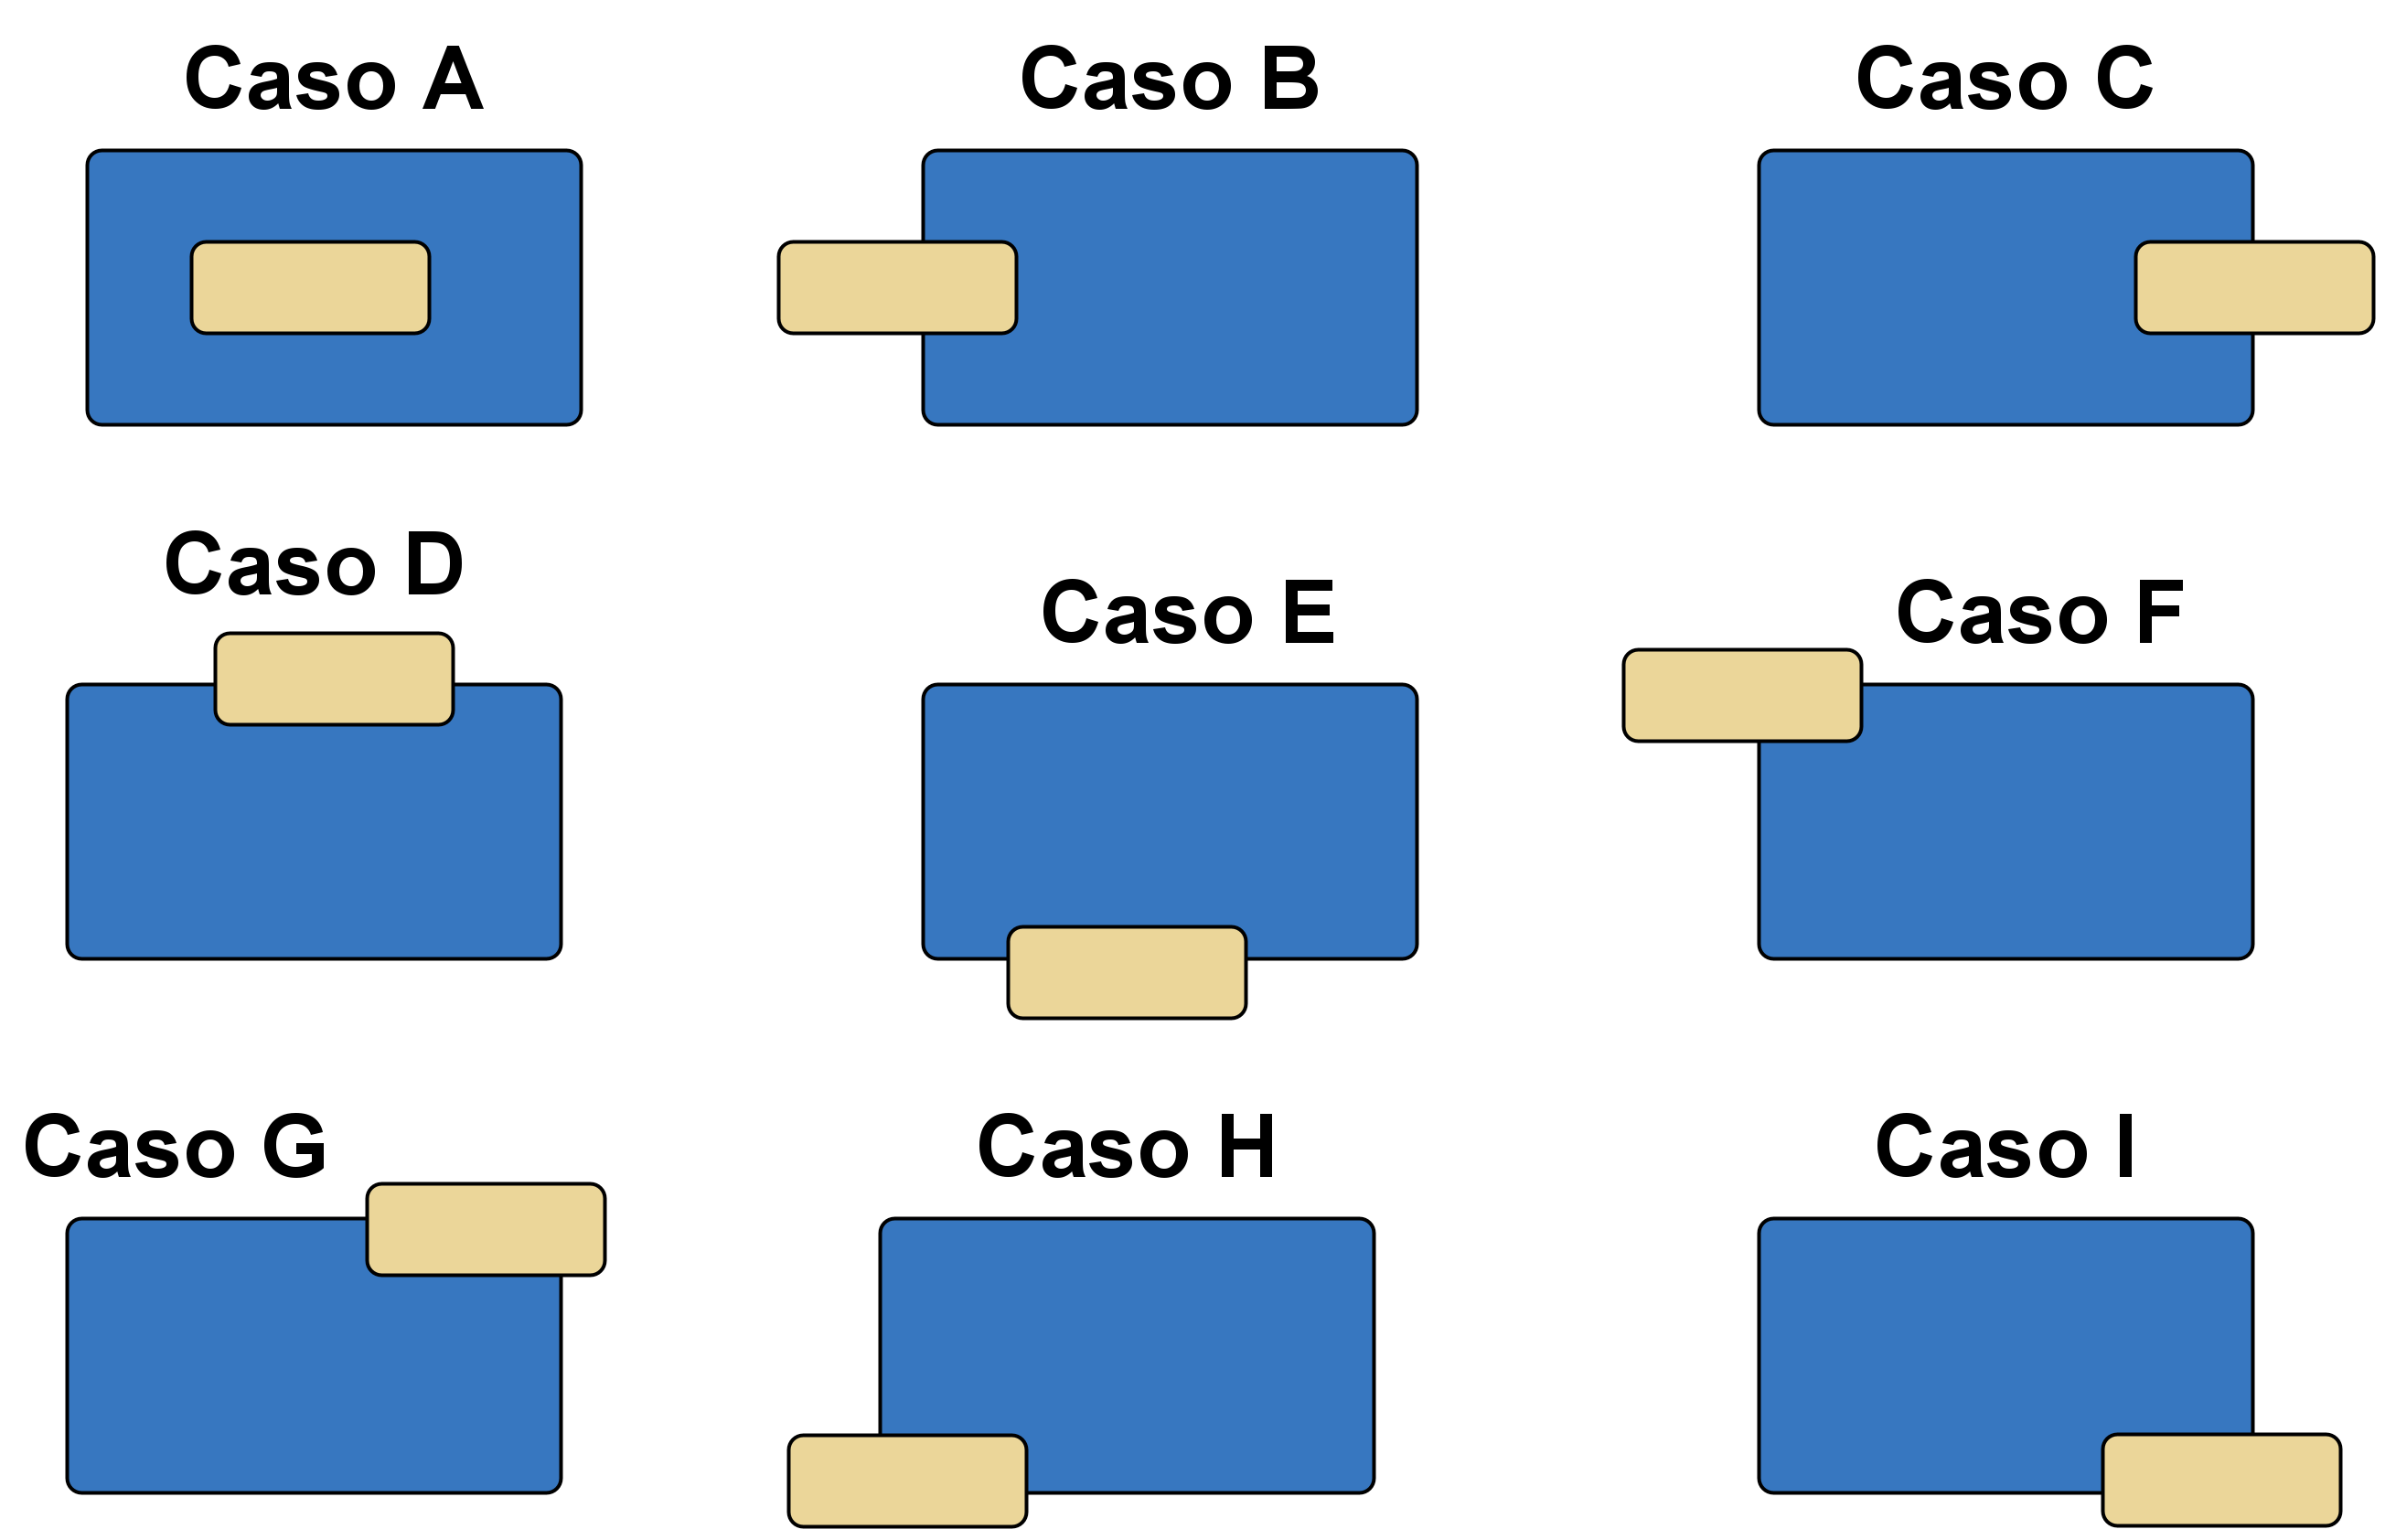
\includegraphics[width=0.8\textwidth]{imaxes/z-adicional/casos-algoritmo-seleccion-regiones.png}
    \caption{Casos considerados en el algoritmo de selección de regiones}
    \label{fig:casos-algoritmo-seleccion-regiones}
\end{figure}

\begin{figure}[hp!]
	\centering
	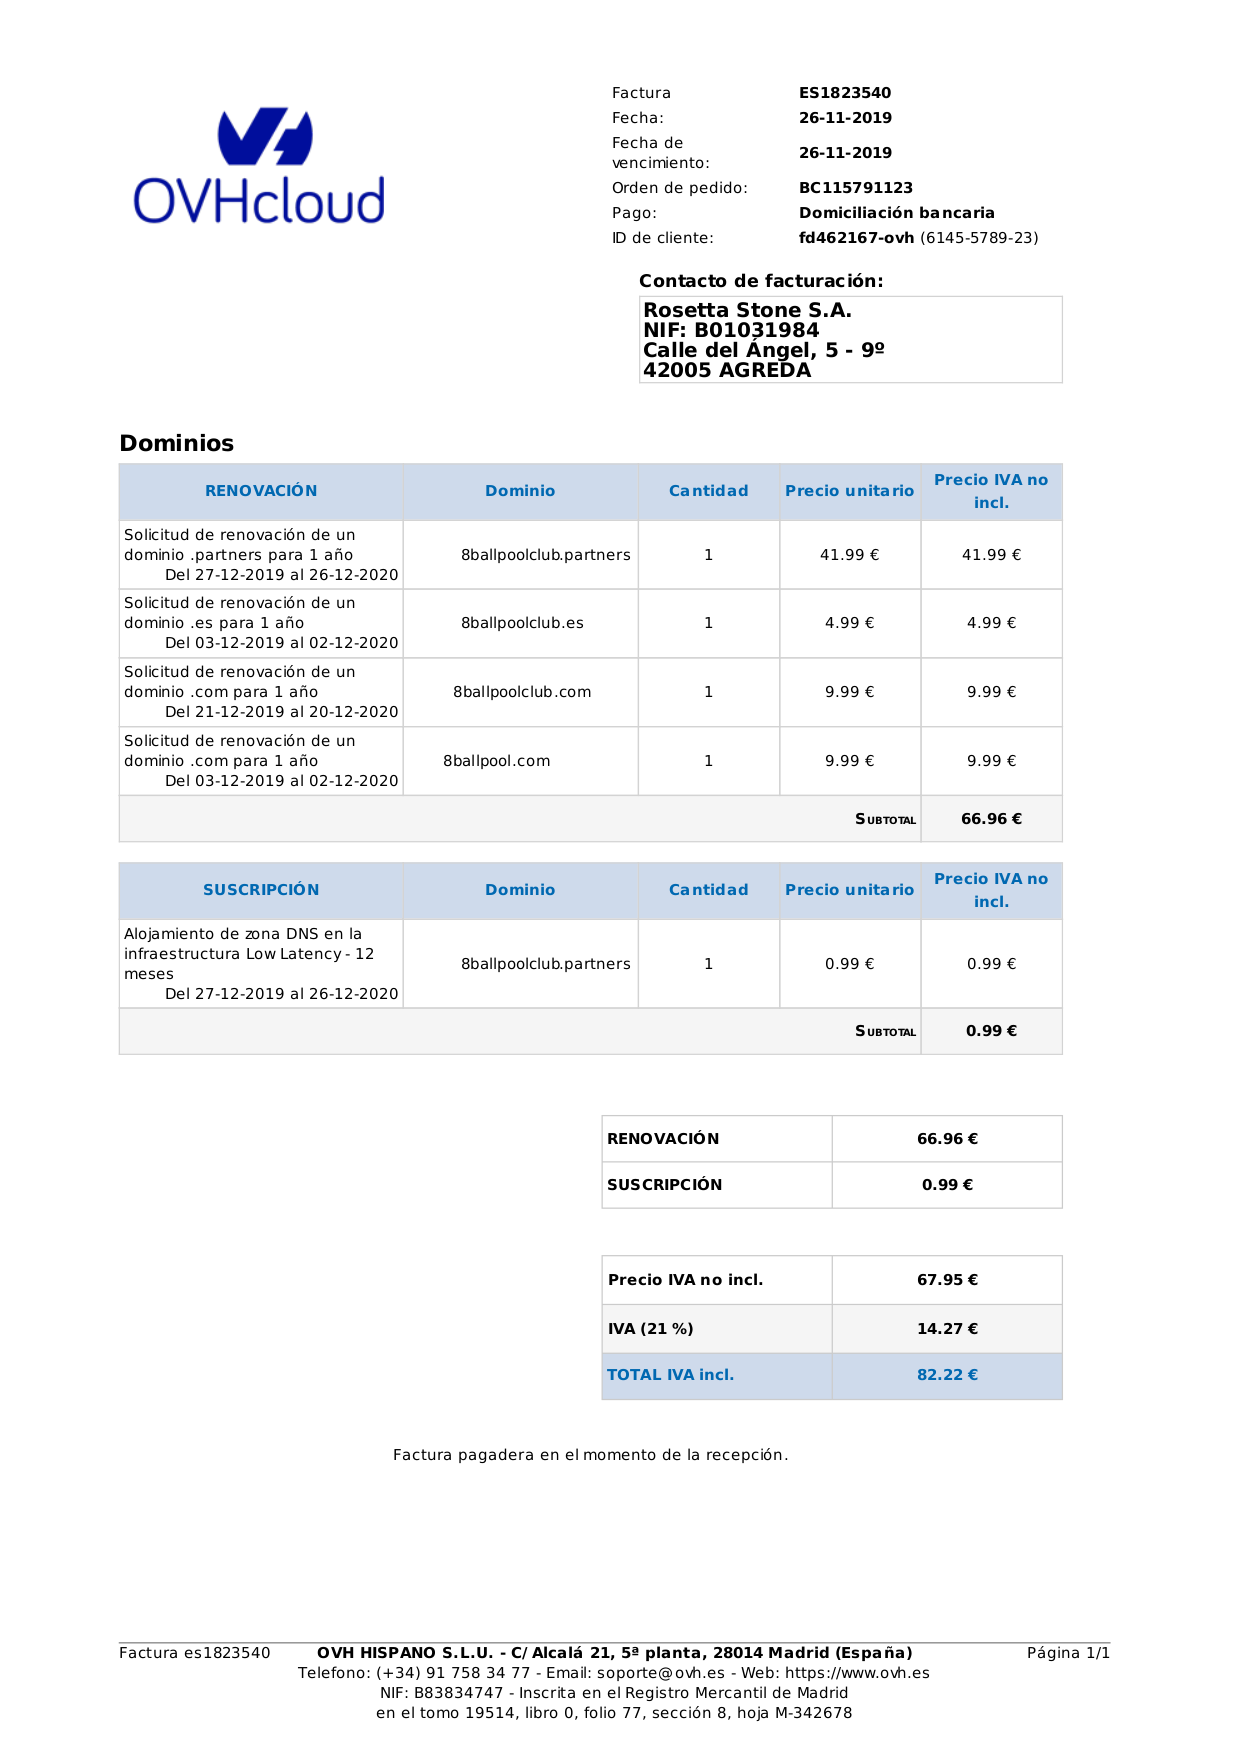
\includegraphics[angle=0,height=1.4\textwidth]{imaxes/z-adicional/modelo-ovh}
	\caption{Ejemplo de modelo de OVH}
	\label{fig:modelo-ovh}
\end{figure}

\begin{figure}[hp!]
	\centering
	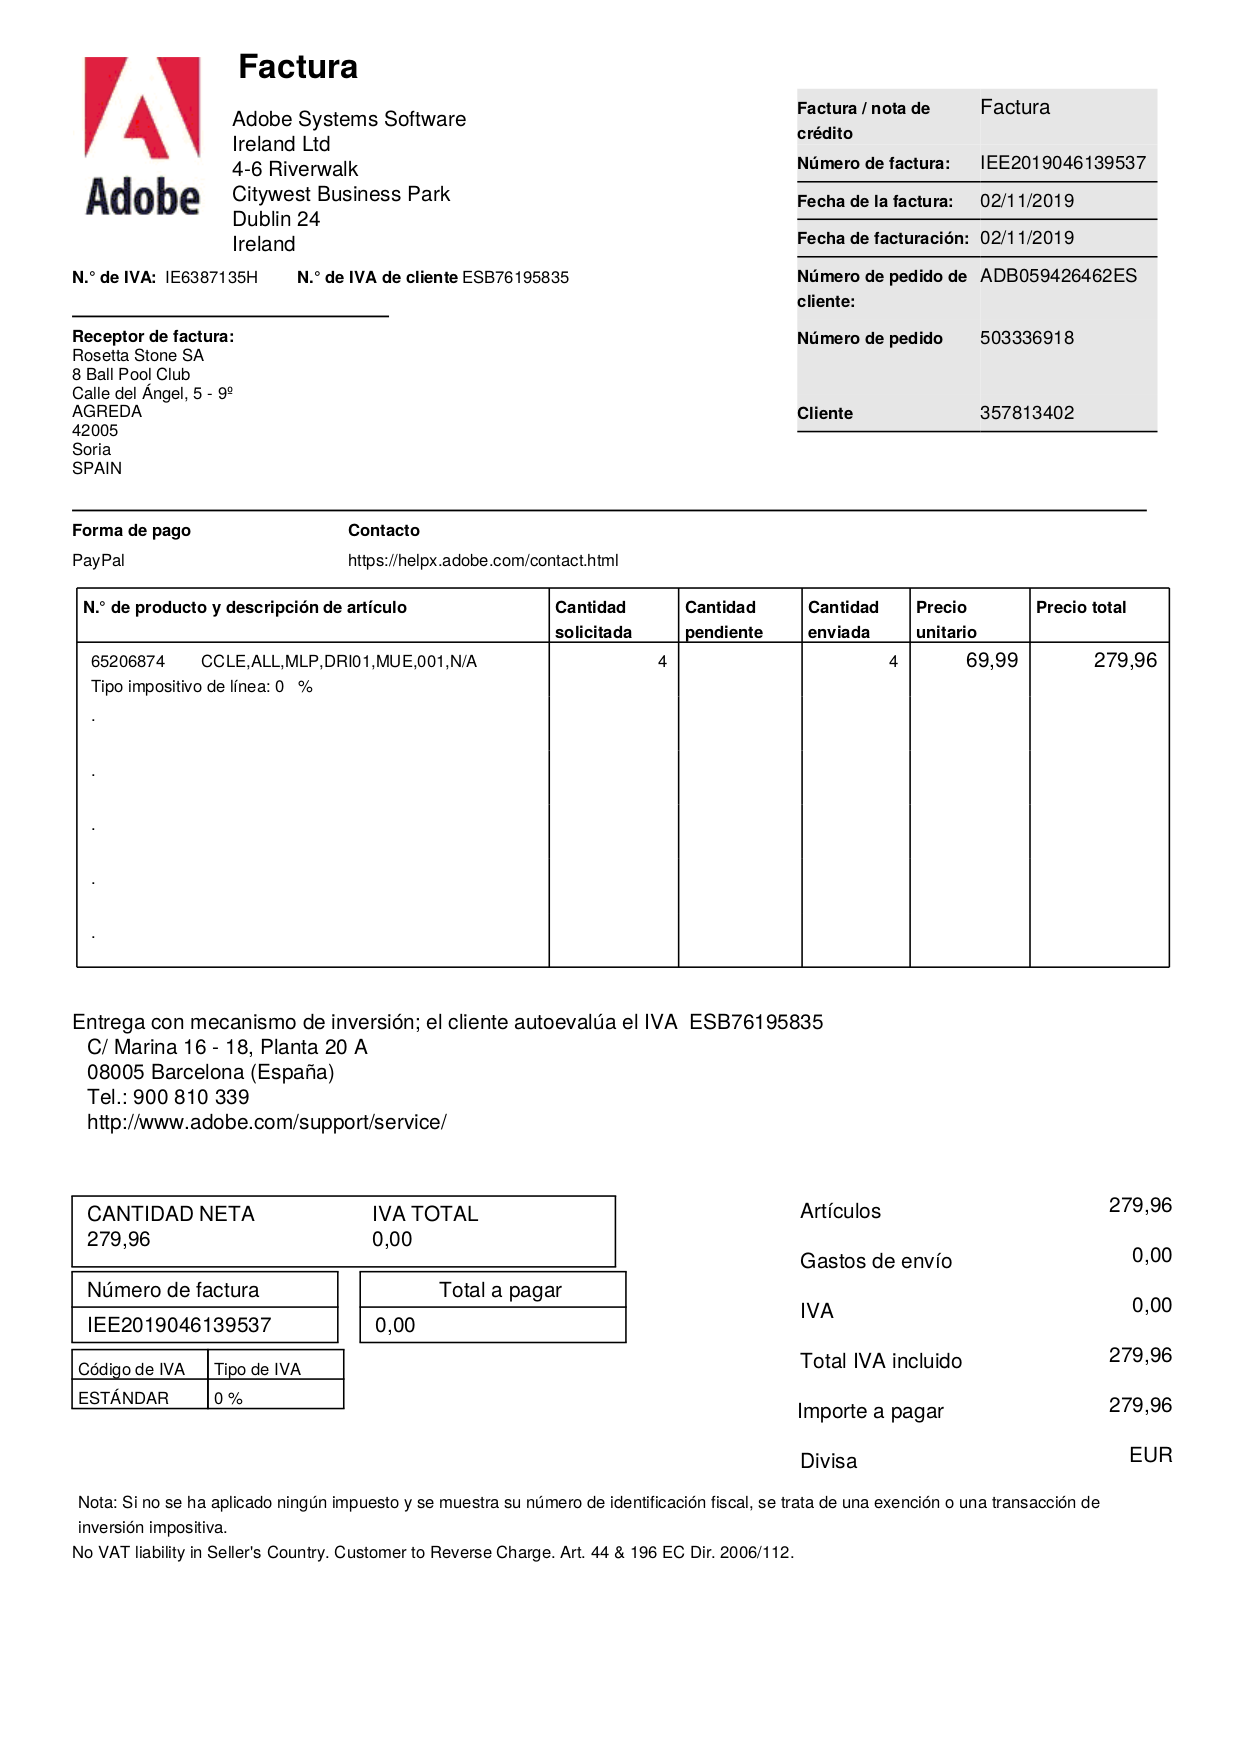
\includegraphics[angle=0,height=1.4\textwidth]{imaxes/z-adicional/modelo-adobe}
	\caption{Ejemplo de modelo de Adobe}
	\label{fig:modelo-adobe}
\end{figure}

\begin{figure}[hp!]
	\centering
	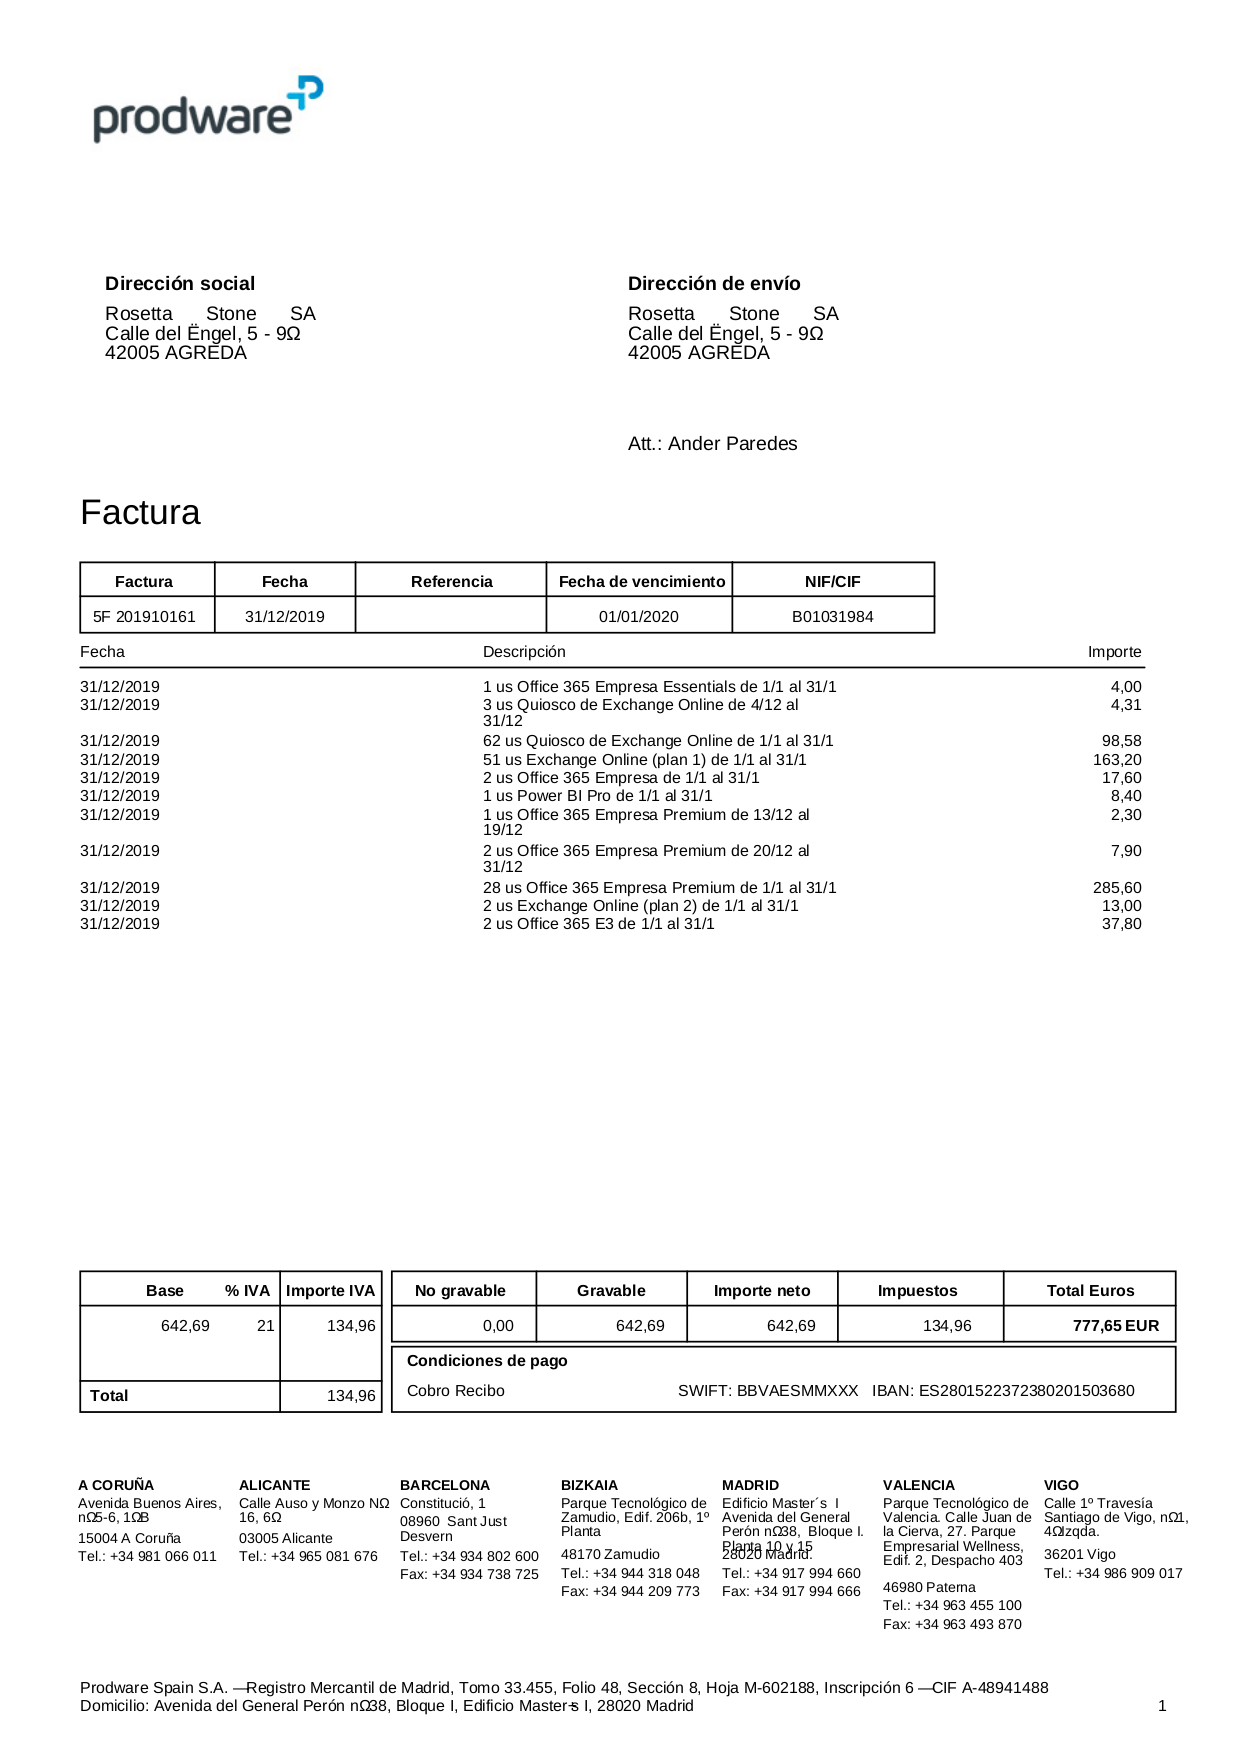
\includegraphics[angle=0,height=1.4\textwidth]{imaxes/z-adicional/modelo-prodware}
	\caption{Ejemplo de modelo de Prodware}
	\label{fig:modelo-prodware}
\end{figure}

\begin{figure}[hp!]
	\centering
	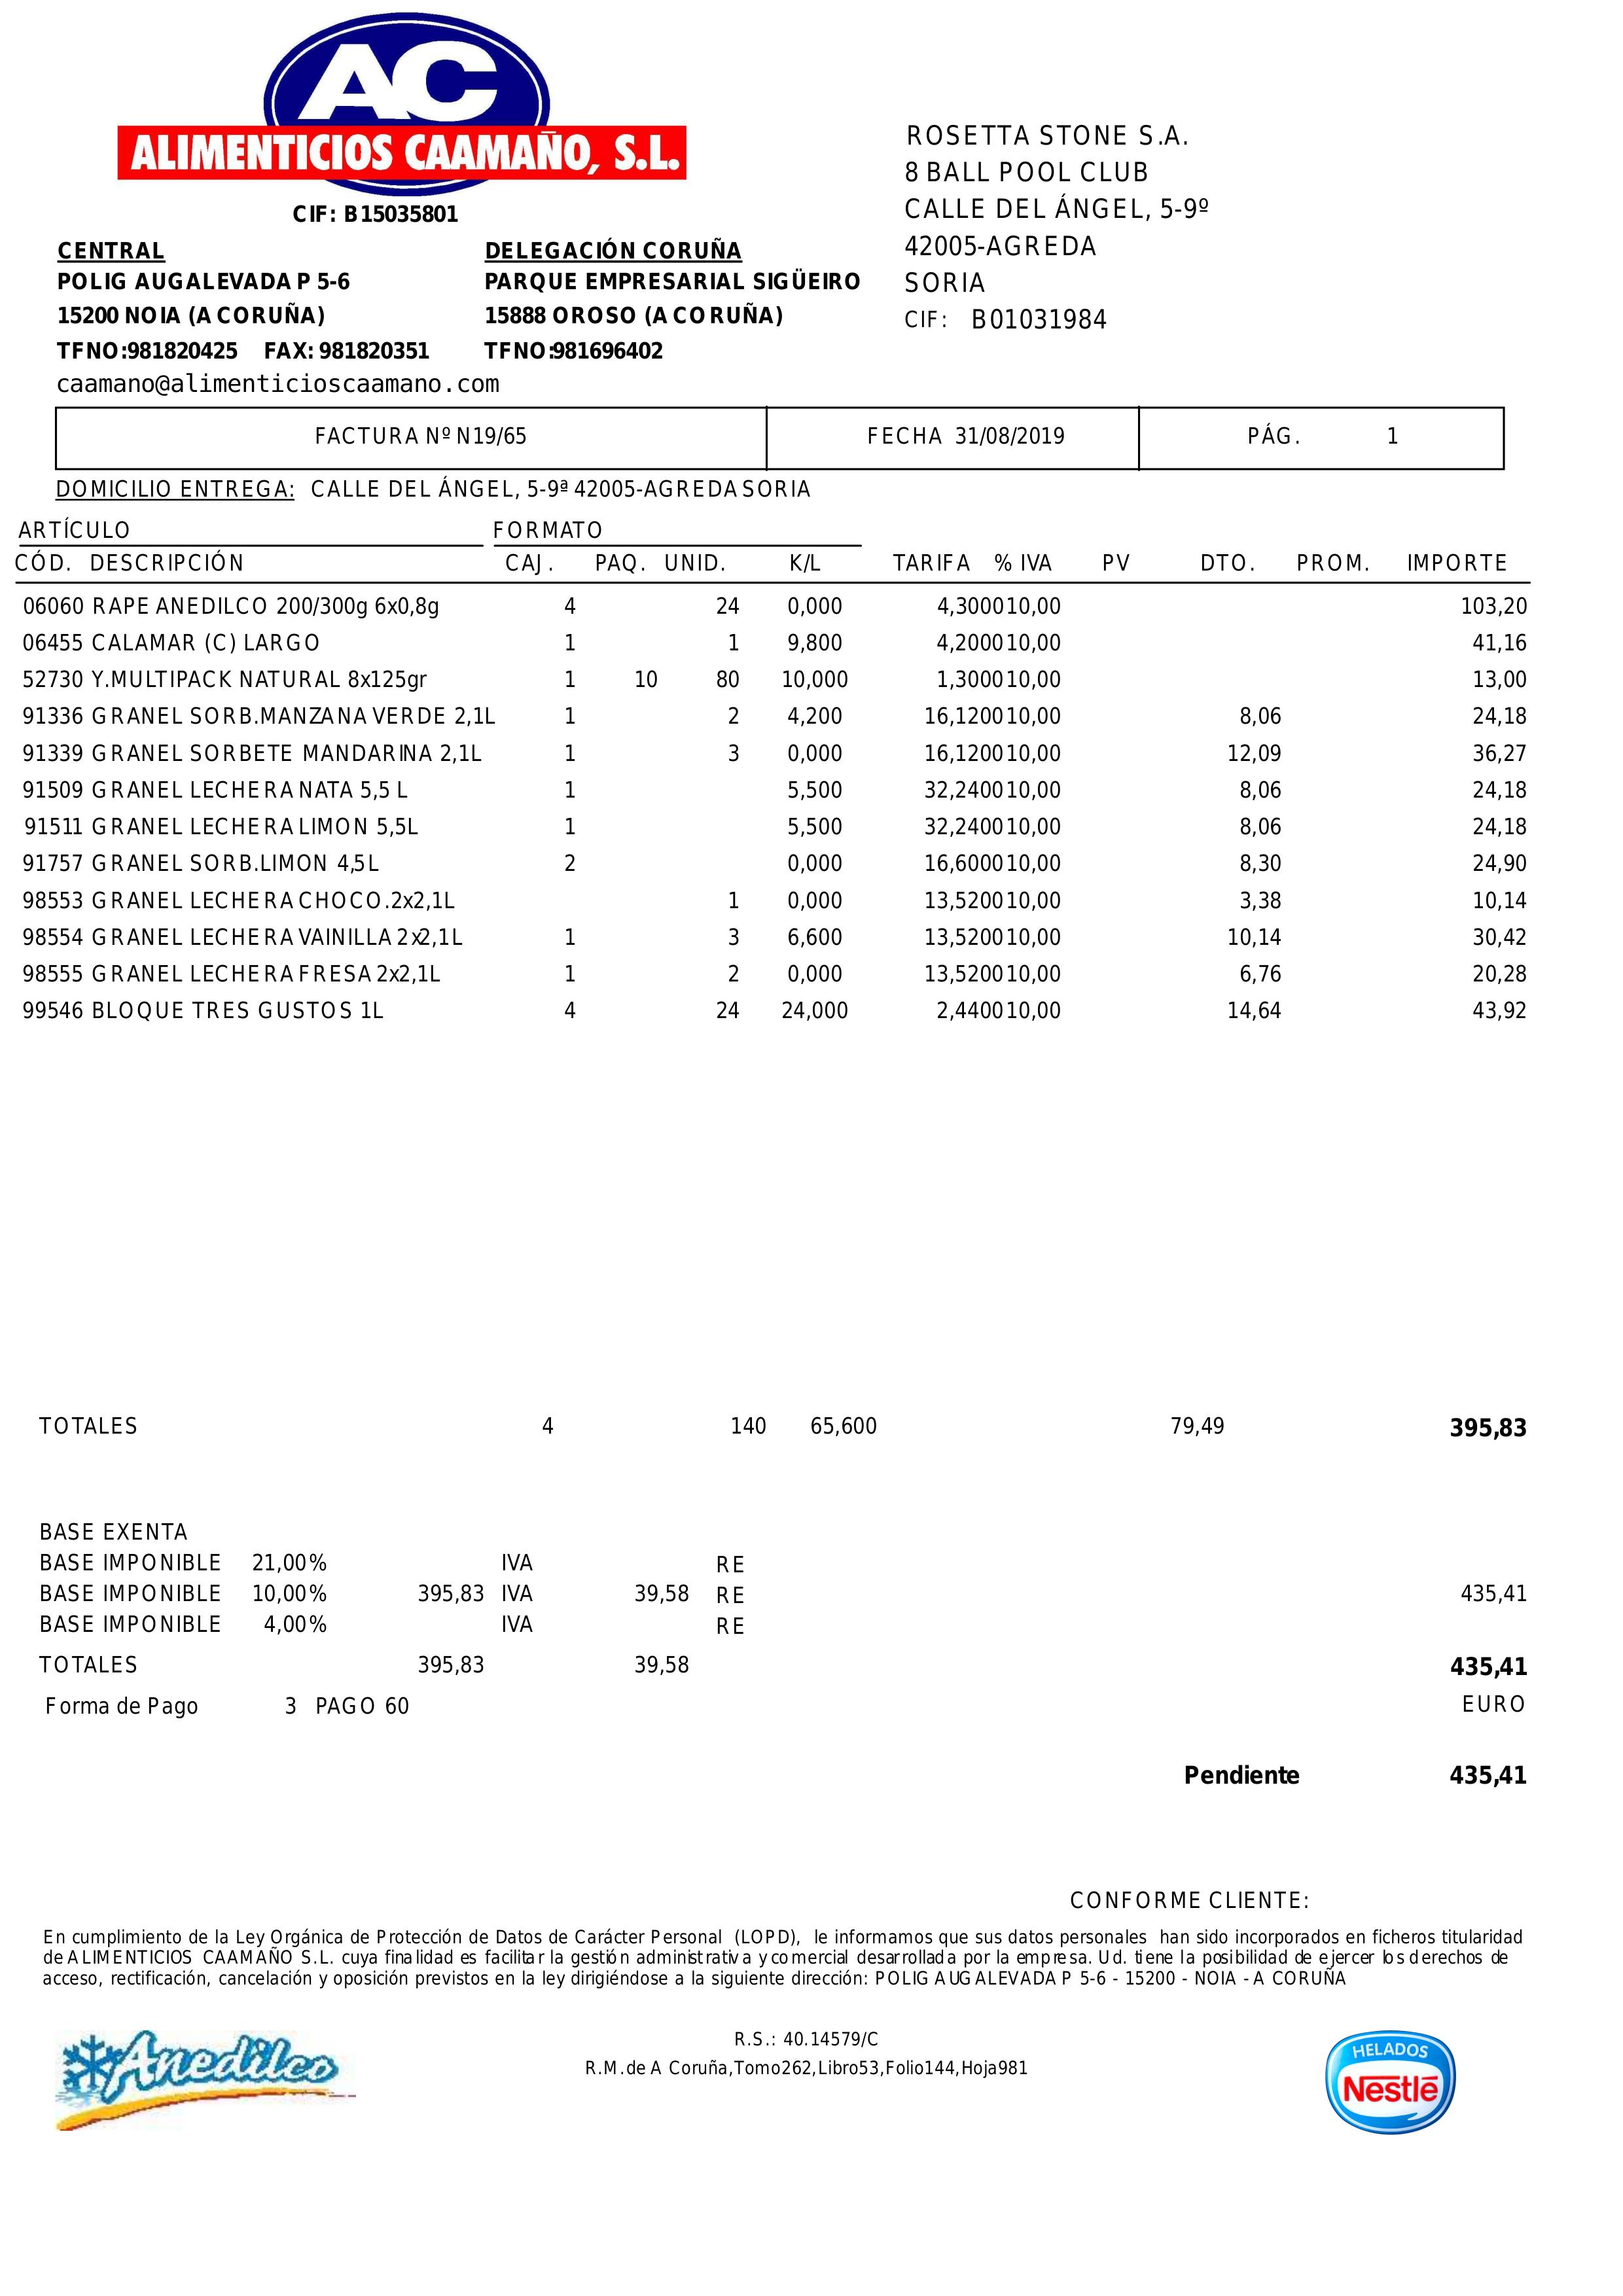
\includegraphics[angle=0,height=1.4\textwidth]{imaxes/z-adicional/modelo-ac}
	\caption{Ejemplo de modelo de AC}
	\label{fig:modelo-ac}
\end{figure}